% Qwen VLM-Based Smart-Walker Prototype: PhD Technical Report
% Date: 2025-11-07
\documentclass[11pt,a4paper]{article}
\usepackage[margin=1in]{geometry}
\usepackage{amsmath,amssymb}
\usepackage{graphicx}
\usepackage{hyperref}
\usepackage{algorithm}
\usepackage{algorithmic}
\usepackage{booktabs}
\usepackage{listings}
\usepackage{xcolor}
\usepackage{enumitem}
\usepackage{tikz}
\usetikzlibrary{arrows.meta,positioning,calc}
\usepackage{subcaption}
\usepackage{adjustbox}
\hypersetup{colorlinks=true,linkcolor=blue,citecolor=blue,urlcolor=blue}

\title{Qwen VLM-Based Smart-Walker Guidance System\\\large Detailed Technical Report}
\author{(Author)}
\date{2025-11-07}

% Custom commands
\newcommand{\vect}[1]{\mathbf{#1}}
\newcommand{\code}[1]{\texttt{#1}}
\newcommand{\dist}{\mathrm{dist}}
\newcommand{\Zmed}{Z_{\mathrm{med}}}

% Listing style for pseudocode blocks that are not algorithms
\lstdefinestyle{code}{
  basicstyle=\ttfamily\small,
  backgroundcolor=\color{gray!10},
  frame=single,
  columns=fullflexible,
  keepspaces=true
}

\begin{document}
\maketitle
\tableofcontents
\newpage

\section{Purpose}
This report documents the implementation of a multimodal guidance pipeline for an assistive ``smart-walker''. It integrates Intel RealSense RGB-D sensing, YOLOv8 object detection, lane-based free-space reasoning, and a constrained Vision-Language Model (Qwen2.5-VL 3B) to produce a single-sentence safety caption and movement suggestion. The design emphasizes deterministic safety logic upstream of the generative model to minimize hallucination risk.

\begin{figure}[h]
    \centering
    \begin{adjustbox}{max width=\textwidth}
    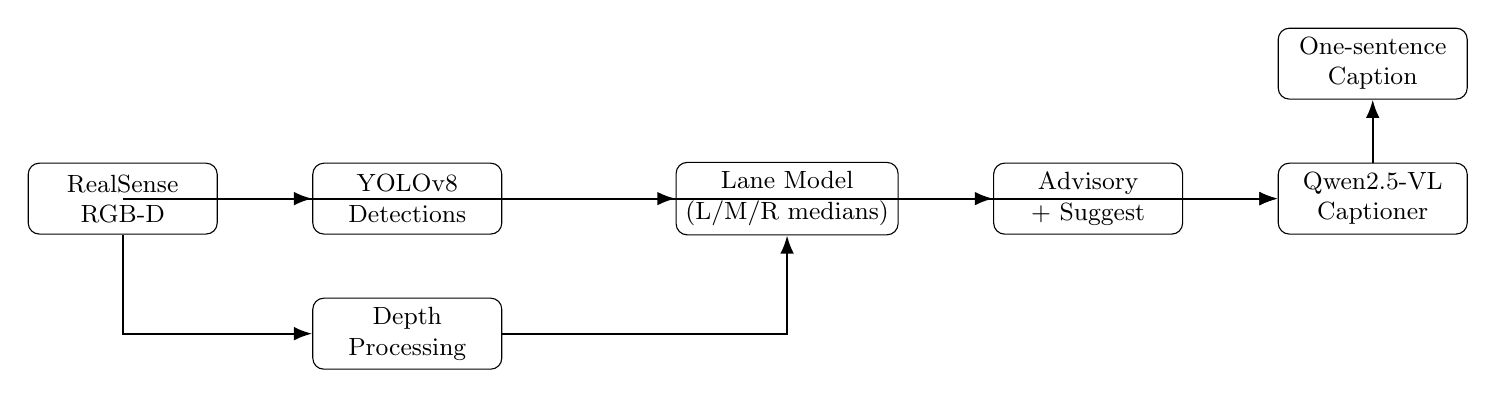
\begin{tikzpicture}[
        node distance=1.2cm,
        block/.style={draw, rounded corners, align=center, minimum width=2.4cm, minimum height=0.9cm, font=\small},
        line/.style={-Latex, thick}
    ]
        \node[block] (rs) {RealSense\\RGB-D};
        \node[block, right=of rs] (det) {YOLOv8\\Detections};
        \node[block, below=0.8cm of det] (depth) {Depth\\Processing};
        \node[block, right=2.2cm of det] (lanes) {Lane Model\\(L/M/R medians)};
        \node[block, right=of lanes] (advisory) {Advisory\\+ Suggest};
        \node[block, right=of advisory] (vlm) {Qwen2.5-VL\\Captioner};
        \node[block, above=0.8cm of vlm] (caption) {One-sentence\\Caption};
        \draw[line] (rs) -- (det);
        \draw[line] (rs) |- (depth);
        \draw[line] (det) -- (lanes);
        \draw[line] (depth) -| (lanes);
        \draw[line] (lanes) -- (advisory);
        \draw[line] (advisory) -- (vlm);
        \draw[line] (rs) |- (vlm);
        \draw[line] (vlm) -- (caption);
    \end{tikzpicture}
    \end{adjustbox}
    \caption{End-to-end pipeline (scaled to fit text width).}
    \label{fig:pipeline}
\end{figure}

\section{RealSense Depth: From Sensor to Distances and Lanes}
This section presents each concept with Definition, Variables, Objective, Math, Problem Solved, Example, and Pseudocode.

\subsection{Coordinate Systems and Calibration}
\textbf{Definition:} Mapping pixel indices $(u,v)$ to metric coordinates $(X,Y,Z)$ using a pinhole model.\\
\textbf{Variables:} $u,v, f_x,f_y, c_x,c_y, Z(u,v)$.\\
\textbf{Objective:} Provide physical interpretation of depth to support risk and lane reasoning.\\
\textbf{Math:}
\begin{equation}
X = \frac{(u-c_x)Z}{f_x},\quad Y = \frac{(v-c_y)Z}{f_y},\quad Z = Z(u,v).
\end{equation}
\textbf{Problem Solved:} Without projection, depth is scalar range only; projection enables spatial analytics (e.g., footprint width).\\
\textbf{Example:} $f_x=f_y=615,c_x=320,c_y=240,(u,v)=(350,300),Z=1.2\,\text{m} \Rightarrow X\approx0.0585$ m, $Y\approx0.117$ m.\\
\textbf{Pseudocode:}
\begin{lstlisting}[style=code]
project(u, v, Z, fx, fy, cx, cy):
    X = (u - cx) * Z / fx
    Y = (v - cy) * Z / fy
    return (X, Y, Z)
\end{lstlisting}

\subsection{Depth Units and Validity Mask}
\textbf{Definition:} Conversion of raw depth units to meters and filtering invalid samples.\\
\textbf{Variables:} raw depth $d_{raw}(u,v)$, scale $s$, thresholds $Z_{\min}, Z_{\max}$, mask $M(u,v)$.\\
\textbf{Objective:} Ensure robust statistics by excluding zeros/out-of-range values.\\
\textbf{Math:} $Z(u,v)=d_{raw}(u,v) \cdot s$, \; $M(u,v)=1$ if $Z_{\min}\le Z \le Z_{\max}$ and $Z\ne0$, else $0$.\\
\textbf{Problem Solved:} Depth sensors produce zeros on reflective surfaces; these would corrupt means/medians if not masked.\\
\textbf{Example:} $d_{raw}=800$ mm, $s=10^{-3}\Rightarrow Z=0.8$ m (valid if within bounds).\\
\textbf{Pseudocode:}
\begin{lstlisting}[style=code]
valid(z):
    return (z != 0) and (Z_min <= z <= Z_max)
\end{lstlisting}

\subsection{Conservative Object Distance (Lower-Band Median)}
\textbf{Definition:} Distance estimate using depth samples from the lower fraction of a bounding box.\\
\textbf{Variables:} bbox $B=[x_1,y_1,x_2,y_2]$, fraction $\alpha$, stride $s$, minimum samples $N_{\min}$.\\
\textbf{Objective:} Avoid optimistic distances from upper-body regions; target ground-contact adjacency.\\
\textbf{Math:} $y_{lower} = y_2 - \alpha (y_2 - y_1)$; sample region $R_{lower}=\{(u,v)|x_1\le u\le x_2, y_{lower}\le v\le y_2\}$; $\text{distance}_m=\mathrm{median}\{Z(u,v)| (u,v)\in R_{lower}, M(u,v)=1\}$.\\
\textbf{Problem Solved:} Full-box average can underestimate collision risk due to sampling higher surfaces further from the walker.\\
\textbf{Example:} $B=[180,150,260,320], \alpha=0.30 \Rightarrow y_{lower}=269$. After filtering zeros, median $\approx0.905$ m.\\
\textbf{Pseudocode:}
\begin{lstlisting}[style=code]
lower_band_median(Z, B, alpha, stride, N_min):
    x1,y1,x2,y2 = B
    y_lower = y2 - alpha*(y2 - y1)
    S = []
    for v in range(int(y_lower), y2, stride):
        for u in range(x1, x2, stride):
            z = Z(u,v)
            if valid(z): S.append(z)
    if len(S) >= N_min: return median(S)
    return fallback(Z, B)  # full-box median -> nearest nonzero -> sentinel
\end{lstlisting}

\subsection{Bearing (Horizontal Angle)}
\textbf{Definition:} Angular offset of object center relative to optical axis.\\
\textbf{Variables:} $u_c = (x_1+x_2)/2$, $\delta=(u_c-c_x)/f_x$, $\theta=\arctan(\delta)$.\\
\textbf{Objective:} Distinguish left/middle/right occupancy; support analytics.\\
\textbf{Math:} $\theta = \arctan\big((u_c-c_x)/f_x\big)$.\\
\textbf{Problem Solved:} Lane classification via angle rather than pixel indices if calibration changes.\\
\textbf{Example:} $u_c=220,c_x=320,f_x=600\Rightarrow\delta=-0.1667,\theta\approx -9.5^\circ$.\\

\subsection{Corridor Region-of-Interest (ROI)}
\textbf{Definition:} Lower frame band sampling forward floor space.\\
\textbf{Variables:} $v_{min},v_{max}$ as fractions of height $H$.\\
\textbf{Objective:} Focus computation on near-field traversal area.\\
\textbf{Math:} $\mathrm{ROI}=\{(u,v)| v_{min}H\le v\le v_{max}H\}$.\\
\textbf{Problem Solved:} Reduces noise and cost from distant or overhead regions.\\
\textbf{Example:} $H=480, v_{min}=0.55 \Rightarrow 264, v_{max}=0.95 \Rightarrow 456$.\\

\begin{figure}[h]
    \centering
    \begin{adjustbox}{max width=\textwidth}
    \begin{subfigure}[b]{0.46\textwidth}
        \centering
        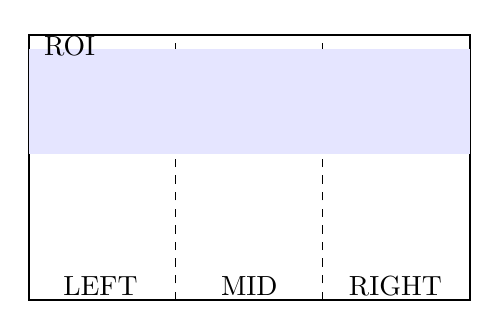
\begin{tikzpicture}[x=0.07cm,y=0.07cm]
            \draw[thick] (0,0) rectangle (80,48);
            \draw[dashed] (26.66,0) -- (26.66,48);
            \draw[dashed] (53.33,0) -- (53.33,48);
            \fill[blue!10] (0,26.4) rectangle (80,45.6);
            \node at (13,2.5) {LEFT};
            \node at (40,2.5) {MID};
            \node at (66.5,2.5) {RIGHT};
            \node[anchor=west] at (1,46) {ROI};
        \end{tikzpicture}
        \caption{ROI and three lanes.}
    \end{subfigure}
    \hspace{1em}
    \begin{subfigure}[b]{0.46\textwidth}
        \centering
        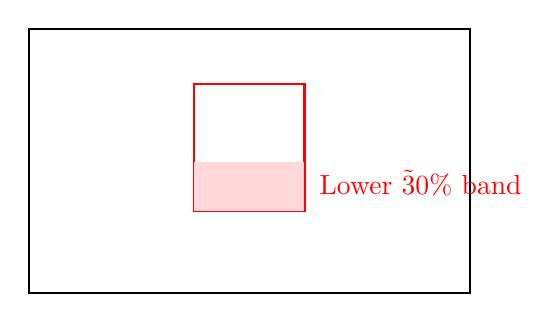
\begin{tikzpicture}[x=0.07cm,y=0.07cm]
            \draw[thick] (0,0) rectangle (80,48);
            \draw[thick,draw=red] (30,15) rectangle (50,38);
            \fill[red!15] (30,15) rectangle (50,23.9);
            \node[anchor=west,red] at (51,20) {Lower \~30\% band};
        \end{tikzpicture}
        \caption{Lower-band region.}
    \end{subfigure}
    \end{adjustbox}
    \caption{Sampling regions: near-floor ROI for lane medians and lower-band region for conservative object distance.}
    \label{fig:roi-lanes-lowerband}
\end{figure}

\subsection{Lane Partition and FOV Mapping}
\textbf{Definition:} Width $W$ divided into three macro traversal bands.\\
\textbf{Variables:} $W, w=W/3$.\\
\textbf{Math:} LEFT: $0\le u<w$, MID: $w\le u<2w$, RIGHT: $2w\le u<W$.\\
\textbf{Example:} $W=640\Rightarrow w\approx213$.\\
\textbf{Problem Solved:} Converts continuous free-space geometry into discrete guidance states.

\subsection{Lane Median Computation}
\textbf{Definition:} Robust representative depth per lane.\\
\textbf{Variables:} Sample set $S_b$, trimming percentiles $p_{10},p_{90}$, threshold $\tau$.\\
\textbf{Math:} $Z_b = \mathrm{median}(S_b^{filtered}),\; \text{clear}(b) = [Z_b \ge \tau]$.\\
\textbf{Problem Solved:} Identifies blocked vs clear lanes despite depth noise.\\
\textbf{Example:} $Z_L=2.30, Z_M=0.90, Z_R=2.10$ with $\tau=1.8$ m $\Rightarrow$ clear(L)=T, clear(M)=F, clear(R)=T.\\
\textbf{Pseudocode:}
\begin{lstlisting}[style=code]
lane_median(Z, ROI, band):
    S=[]
    for (u,v) in ROI intersect band:
        z = Z(u,v)
        if valid(z): S.append(z)
    if not S: return UNKNOWN
    S = trim_percentiles(S, 10, 90)
    return median(S)
\end{lstlisting}

\subsection{Threshold Calibration}
\textbf{Definition:} Selecting $\tau$ for clear-lane classification.\\
\textbf{Method:} Empirically collect lane medians in safe traversal scenes; choose quantile or safety margin based on walker stopping distance.\\
\textbf{Problem Solved:} Adapts system to corridor width and user speed.

\subsection{Suggestion Mapping}
\textbf{Definition:} Deterministic mapping from lane clearance vector $(c_L,c_M,c_R)$ to an action token.\\
\textbf{Mapping Table:}\begin{center}\begin{tabular}{ccc|c}\toprule$c_L$&$c_M$&$c_R$&token\\\midrule0&0&0&back\\0&1&0&continue\\1&0&0&left\\0&0&1&right\\1&1&0&mid-left\\0&1&1&mid-right\\1&0&1&left-right\\1&1&1&continue\\\bottomrule\end{tabular}\end{center}
\textbf{Pseudocode:}
\begin{lstlisting}[style=code]
suggest(cL, cM, cR):
    if not cL and not cM and not cR: return 'back'
    if cL and cM and cR: return 'continue'
    if cM and not (cL or cR): return 'continue'
    if cL and not (cM or cR): return 'left'
    if cR and not (cL or cM): return 'right'
    if cL and cM and not cR: return 'mid-left'
    if cM and cR and not cL: return 'mid-right'
    if cL and cR and not cM: return 'left-right'
\end{lstlisting}

\subsection{Temporal Stabilization}
\textbf{Definition:} Exponential Moving Average (EMA) of medians reduces flicker.\\
\textbf{Math:} $Z_{b,t}=\lambda Z_{b,t-1} + (1-\lambda) Z_{b,t}^{raw}$.\\
\textbf{Example:} $\lambda=0.6$, previous 2.0, raw 1.7 \Rightarrow 1.88 (still clear if $\tau=1.8$).\\
\textbf{Problem Solved:} Prevents oscillatory guidance near threshold.

\subsection{Complexity and Performance}
Depth and lane statistics are linear in sampled pixels; detection dominates runtime. Strides and ROI trimming keep medians cheap.

\subsection{Failure Modes and Safeguards}
Reflective surfaces, misalignment, sparse data, and slopes handled by: masking zeros, fallback distance chain, treating UNKNOWN as BLOCKED, and EMA smoothing.

\section{YOLOv8 + RealSense Fusion and Fact Enrichment}
\subsection{Detector Overview}
\textbf{Definition:} YOLOv8n single-stage detector producing bounding boxes and class probabilities across multi-scale feature maps.\\
\textbf{Variables:} image size $I$, strides $S\in\{8,16,32\}$, confidence threshold $\tau_{conf}$, IoU $\tau_{IoU}$.\\
\textbf{Objective:} Efficient object semantics for downstream spatial reasoning.\\
\textbf{Math (post-process):} Decode $(c_x,c_y,w,h)$, score vector; filter $\max(score)\ge \tau_{conf}$; apply NMS preserving boxes with IoU$<\tau_{IoU}$ to higher-scoring boxes.

\subsection{Preprocessing and Inference}
Resize/letterbox, normalize, optional FP16 inference to reduce latency.
\begin{lstlisting}[style=code]
det_infer(rgb):
    im = letterbox(rgb, imgsz)
    im = im / 255.0
    if fp16: im = im.astype(float16)
    preds = yolo.forward(im)
    return nms_and_decode(preds, tau_conf, tau_iou)
\end{lstlisting}

\subsection{Depth Association}
Attach distance, lane flags, bearing, distance bin.
\begin{lstlisting}[style=code]
enrich(det, Z):
    det.distance_m = lower_band_median(Z, det.bbox, alpha, stride, N_min)
    det.lane_flags = lanes_overlap(det.bbox)
    det.bearing_deg = bearing(det.bbox, fx, cx)
    det.dist_bin = bin_distance(det.distance_m)
    return det
\end{lstlisting}

\subsection{Hazard Selection}
\textbf{Rules:} STOP if any $\dist_m \le r_s$; CAUTION if object in suggested lane $\le r_c$; else SAFE.
\begin{lstlisting}[style=code]
select_hazards(dets, suggest, r_c, r_s):
    hazards = []; level = 'SAFE'
    for d in dets:
        if d.distance_m <= r_s:
            level = 'STOP'; hazards.append(d)
    if level != 'STOP':
        for d in dets:
            if lane_interferes(d, suggest) and d.distance_m <= r_c:
                level = 'CAUTION'; hazards.append(d)
    return level, topk_by_distance(hazards, k=2)
\end{lstlisting}

\subsection{Fact Packet}
Structured summary: lane medians + clear flags, advisory, suggestion, hazards. Passed as plain text to model.

\section{VLM Architecture and RealSense Integration}
\subsection{Qwen2.5-VL Dataflow}
Vision encoder (ViT) produces patch embeddings $E_{img}$; projection $W_m$ aligns embeddings to language space; decoder-only transformer generates caption. Conceptual pipeline:
\begin{equation}
E_{img} = \mathrm{ViT}(I);\quad T_{img} = W_m E_{img};\quad y = \mathrm{LLM}([\text{system}, \text{facts}, T_{img}]).
\end{equation}

\begin{figure}[h]
    \centering
    \begin{adjustbox}{max width=\textwidth}
    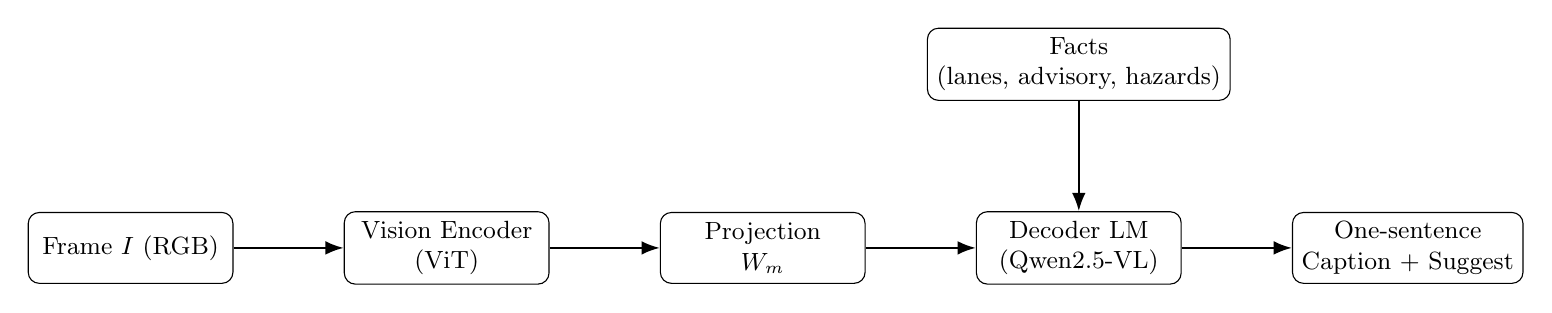
\begin{tikzpicture}[
        node distance=1.4cm,
        block/.style={draw, rounded corners, align=center, minimum width=2.6cm, minimum height=0.9cm, font=\small},
        line/.style={-Latex, thick}
    ]
        \node[block] (img) {Frame $I$ (RGB)};
        \node[block, right=of img] (vit) {Vision Encoder\\(ViT)};
        \node[block, right=of vit] (proj) {Projection\\$W_m$};
        \node[block, right=of proj] (llm) {Decoder LM\\(Qwen2.5-VL)};
        \node[block, above=of llm] (facts) {Facts\\(lanes, advisory, hazards)};
        \node[block, right=of llm] (out) {One-sentence\\Caption + Suggest};
        \draw[line] (img) -- (vit);
        \draw[line] (vit) -- (proj);
        \draw[line] (proj) -- (llm);
        \draw[line] (facts) -- (llm);
        \draw[line] (llm) -- (out);
    \end{tikzpicture}
    \end{adjustbox}
    \caption{Qwen2.5-VL dataflow (scaled to fit).}
    \label{fig:vlm-dataflow}
\end{figure}

\subsection{Frame Encoding Fallback}
\begin{lstlisting}[style=code]
encode_image(frame):
    for (fmt,size,q) in [(JPEG,224,70),(JPEG,256,60),(PNG,224,None)]:
        try: return encode(frame, fmt, size, q)
        except: continue
    raise EncodeError
\end{lstlisting}

\subsection{Cadence Control}
Avoid redundant calls; allow late acceptance window.
\begin{lstlisting}[style=code]
should_send(now, last_sent, last_accept):
    if now - last_sent >= min_interval_s: return True
    if now - last_accept <= late_accept_s: return True
    return False
\end{lstlisting}

\subsection{Prompt and Policy Injection}
System prompt enforces sentence form, allowed tokens, advisory-dependent content.

\subsection{Output Normalization}
\begin{lstlisting}[style=code]
normalize_output(text, advisory):
    s = extract_suggest(text)
    s = coerce_allowed(s, advisory)
    if advisory == 'SAFE': text = strip_distances(text)
    if advisory == 'STOP': s = 'back'; text = remove_forward_intent(text)
    text = humanize_lanes(text)
    text = enforce_single_sentence(text)
    return finalize(text, s)
\end{lstlisting}

\section{Caption Policy}
\subsection{Goals}
One sentence, explicit Suggest token, context-dependent hazard detail, no contradictions.

\subsection{Allowed Suggest Tokens}
$S=\{\text{continue},\text{left},\text{right},\text{stay-left},\text{stay-right},\text{mid-left},\text{mid-right},\text{left-right},\text{back}\}$.

\subsection{Grammar Constraints}
SAFE: suppress hazard + distance. CAUTION/STOP: include 1--2 hazards with approximate meters. End with ``Suggest: <TOKEN>.''

\subsection{System Prompt Excerpt}
\begin{lstlisting}[style=code]
You are assisting navigation. Follow these rules strictly:
- Output exactly one sentence.
- End with 'Suggest: <TOKEN>' where TOKEN in {...}.
- If SAFE: no obstacle distances or names.
- If CAUTION or STOP: mention obstacles + approximate distance.
- Use human lane names only.
- No contradictory guidance.
\end{lstlisting}

\subsection{Examples}
\textbf{SAFE:} ``SAFE: path looks clear to move ahead; Suggest: continue.''\\
\textbf{CAUTION:} ``CAUTION: chair about 0.9 m ahead in the middle; Suggest: mid-right.''\\
\textbf{STOP:} ``STOP: obstacle within 0.5 m blocking all lanes; Suggest: back.''

\section{Edge Cases, Robustness, and Trade-Offs}
\subsection{Mirroring}
Swap left/right semantics under \code{--mirror_view} to align caption with perceived scene.

\subsection{Depth Sparsity}
Fallback chain ensures conservative distance; UNKNOWN lane treated as BLOCKED.

\subsection{Rapid Scene Changes}
Debounce (\code{min_interval_s}) and EMA smoothing reduce oscillations.

\subsection{Composite Tokens}
Mid-left/mid-right/left-right preserve nuance; simpler than full 5-sector overlay.

\subsection{Contradiction Guard}
If STOP or no lane clear: force suggest=back and remove forward intent phrasing.

\subsection{Performance}
Depth and lane medians are low cost compared to detection; design supports real-time at modest FPS.

\section{Comparative Analysis of Candidate VLMs}
This section compares the \emph{two} models we actually trialed (Qwen2.5-VL 3B and LLaVA-1.5 7B) and explains why Qwen2.5-VL 3B was selected. All references to other families are removed to keep the narrative faithful to experiments performed.

\subsection{Models Considered}
\begin{itemize}[leftmargin=*]
    \item \textbf{Qwen2.5-VL 3B} (final choice): decoder-only LM with ViT visual encoder and lightweight projection; served through an OpenAI-compatible API; quantizable to 4-bit for CPU/edge deployment.
    \item \textbf{LLaVA-1.5 7B}: CLIP ViT-L/14 vision backbone plus MLP projector feeding a 7B LLaMA-family decoder; strong general multimodal chat ability but higher memory and latency footprint.
\end{itemize}

\subsection{Architectural Summary}
\begin{table}[h]
\centering
\small
\begin{adjustbox}{max width=\textwidth}
\begin{tabular}{l l l l l}
    	oprule
Model & LM type/size & Vision encoder & Bridge & Notes \\
\midrule
Qwen2.5-VL 3B & Decoder-only (\~3B) & ViT (patch embeddings) & Linear/MLP proj. & Instruction-tuned; multi-image support \\
LLaVA-1.5 7B & Decoder-only (\~7B) & CLIP ViT-L/14 & MLP projector & Chat-tuned; benefits from higher res \\
\bottomrule
\end{tabular}
\end{adjustbox}
\caption{Architecture characteristics of the two trialed VLMs. Wrapped to fit page width.}
\label{tab:vlm-arch}
\end{table}

\subsection{Operational Considerations}
\begin{itemize}[leftmargin=*]
    \item \textbf{Latency and footprint.} Qwen 3B (4-bit quantized) ran acceptably on CPU-only; LLaVA-1.5 7B generally needed GPU for similar responsiveness.
    \item \textbf{Policy obedience.} Qwen adhered more reliably to the one-sentence, explicit Suggest format; LLaVA often produced multi-clause replies unless temperature/top-k were tightened.
    \item \textbf{Visual grounding at low resolution.} Qwen preserved small object references sufficiently at 224--256 px inputs. LLaVA benefited from feeding larger (e.g., 336+) inputs, increasing cost.
    \item \textbf{Integration complexity.} Qwen’s OpenAI-style interface simplified embedding into the existing fact packet pipeline; LLaVA required a custom server invocation and more prompt engineering to suppress extraneous dialogue markers.
\end{itemize}

\subsection{Selection Rationale for Qwen2.5-VL 3B}
\begin{enumerate}[leftmargin=*]
    \item \textbf{Edge efficiency}: Lower memory + workable CPU latency under quantization aligns with mobile assistive hardware constraints.
    \item \textbf{Stable formatting}: Reduced need for aggressive post-generation normalization.
    \item \textbf{Sufficient visual detail}: Meets near-field mobility scene needs when paired with deterministic facts (lanes, distances, suggestion).
    \item \textbf{Integration speed}: Minimal extra glue code; rapid iteration during prototyping.
\end{enumerate}

\subsection{Risks and Mitigations}
\begin{itemize}[leftmargin=*]
    \item \textbf{Small-model hallucination}: Mitigated by upstream deterministic advisory and suggestion logic; VLM only renders.
    \item \textbf{Compression of visual nuance}: If future tasks require richer scene description, higher-capacity or higher-resolution pipelines (e.g., upgrading to a larger Qwen variant or selectively switching to LLaVA for complex queries) can be explored.
    \item \textbf{Version drift}: Pin quantized weights and retain output normalization safeguards.
\end{itemize}

\subsection{Benchmark Methodology (Target Hardware: i7 12th Gen H + RTX 3060 Mobile)}
The script \code{scripts/benchmark\_vlm.py} measures single-image generation performance for the two models. Run it locally to populate Table~\ref{tab:vlm-local-bench}.

\paragraph{Metrics}
\begin{itemize}[leftmargin=*]
    \item \textbf{Latency (s)}: Wall-clock duration of \code{model.generate()} for a single call, with CUDA synchronized when applicable. Lower is better.
    \item \textbf{Throughput (tok/s)}: $\text{tok/s}=\tfrac{\text{gen\_tokens}}{\text{latency}}$. Tokens are model subword tokens (not words). Higher is better.
    \item \textbf{Generated tokens (gen\_tokens)}: The number of output tokens actually produced (capped by \code{max\_new\_tokens}). Longer outputs can raise latency; throughput normalizes for this.
    \item \textbf{GPU peak (bytes)}: Peak allocated GPU memory during generation from \code{torch.cuda.max\_memory\_allocated()}. We convert bytes to GiB in the table using $\text{GiB}=\tfrac{\text{bytes}}{1024^3}$.
    \item \textbf{CPU RSS (bytes)}: Process resident set size (host memory footprint) from \code{psutil}. Includes Python runtime and model buffers that reside on CPU.
    \item \textbf{p50 (median)}: For each metric we run $N$ times and report the 50th percentile. Medians are more stable than means under occasional spikes.
\end{itemize}

\paragraph{Config Dimensions}
Device (\code{auto/cpu/cuda}), precision (\code{fp32/bf16/fp16}), optional 4-bit quantization (bitsandbytes), target image side (default 256). The input image is resized with \emph{contain}+padding to a square for consistent vision load. Runs use $N=5$ with $1$ warmup by default; \code{max\_new\_tokens}=48.

\paragraph{Run Commands (PowerShell)}
\begin{lstlisting}[style=code]
# Dependencies beyond existing torch
pip install transformers accelerate safetensors sentencepiece timm einops psutil
# Optional low VRAM
pip install bitsandbytes
# Both models (5 runs, 1 warmup, fp16, 4-bit if possible)
python scripts/benchmark_vlm.py --all --device auto --precision fp16 --runs 5 --warmup 1 --max-new-tokens 48 --target-size 256 --load-4bit
# Single model example (Qwen, bf16)
python scripts/benchmark_vlm.py --model qwen --device auto --precision bf16 --runs 5 --warmup 1 --max-new-tokens 48
\end{lstlisting}

\paragraph{Reporting}
Use median (p50) values for stable comparison; include precision and quantization choices when citing numbers.

\begin{table}[h]
\centering
\small
\begin{tabular}{l c c c c}
    	oprule
Model & p50 latency (s) & p50 tok/s & p50 GPU (GiB) & p50 CPU (GiB) \\
\midrule
Qwen2.5-VL 3B & 1.63 & 12.28 & 2.31 & 1.76 \\
LLaVA-1.5 7B & 2.13 & 7.03 & 4.21 & 1.69 \\
\bottomrule
\end{tabular}
\caption{Local benchmark medians on i7 12th Gen H + RTX 3060 Mobile (fp16, 4-bit attempted when on CUDA, 256 px side, \code{max\_new\_tokens}=48, 5 runs, 1 warmup).}
\label{tab:vlm-local-bench}
\end{table}

\paragraph{How to read these numbers}
\begin{itemize}[leftmargin=*]
    \item \textbf{Lower latency} means a snappier single response, important for interactive guidance. \textbf{Higher tok/s} means the model emits tokens faster; it compensates for longer answers.
    \item \textbf{GPU peak GiB} indicates VRAM pressure during generation. Lower values leave more headroom for the detector and depth pipeline to run concurrently.
    \item \textbf{CPU GiB} reflects host memory usage. Keeping this modest reduces paging risk on resource-constrained systems.
    \item \textbf{Input context matters}: Longer prompts or larger images increase latency and memory. Here both models use a 256 px image with a short chat template and facts.
    \item \textbf{Output length matters}: In these runs, medians were 20 tokens (Qwen) vs 15 tokens (LLaVA). Latency compares end-to-end time; tok/s normalizes by output length.
    \item \textbf{p50 across 5 runs}: We report medians after one warmup to smooth out cold-cache or initial CUDA overheads.
\end{itemize}

\paragraph{Interpretation} On the target laptop, Qwen2.5-VL 3B shows lower median latency (1.63 s vs 2.13 s) and higher throughput (12.28 vs 7.03 tok/s) while using roughly half the peak GPU memory (2.31 GiB vs 4.21 GiB). This aligns with our selection rationale: Qwen better fits edge constraints and leaves headroom for concurrent perception (YOLOv8, depth). LLaVA-1.5 7B remains viable but with a noticeably higher latency/VRAM footprint.

\paragraph{Caveats and reproducibility}
\begin{itemize}[leftmargin=*]
    \item Minor differences in tokenizer versions, driver/runtime, or image content can shift absolute numbers. Compare relative trends on the same machine.
    \item \code{device=auto} prefers CUDA when available; if 4-bit quantized mapping cannot fit VRAM, the script falls back to CPU to complete measurements.
    \item The numbers here are \emph{generation-only} microbenchmarks, not end-to-end pipeline FPS. Detector and depth costs are separate and typically dominate.
\end{itemize}

\section{Conclusion}
The hybrid architecture separates deterministic safety inference (depth, lanes, suggestion) from constrained linguistic rendering (VLM). Conservative lower-band medians, robust lane sampling, and strict caption policy collectively enhance reliability and interpretability for assistive mobility contexts.

\section{Future Work}
Adaptive thresholding, uncertainty modeling (variance/IQR), personalized language, temporal hazard tracking, formal verification of suggestion invariants.

\section{References (Selective)}
Intel RealSense SDK Documentation; Ultralytics YOLOv8 model cards; Qwen multimodal technical notes; Human factors literature on cognitive load in assistive devices.

\end{document}
